%\DocumentMetadata{%
%pdfstandard=A-3b,%
%lang=en,
%}
\documentclass[fontsize=10pt]{datasheet}

% Input encoding and typographical rules for English language
\usepackage{iftex}
\ifPDFTeX
    \usepackage[utf8]{inputenc}
\else
    \ifXeTeX
        \usepackage{fontspec}
    \fi
\fi

\usepackage[english]{babel}
\usepackage[iso,english]{isodate}
\usepackage{siunitx}
\usepackage[subpreambles=true]{standalone}
\usepackage{import}

% hyperref was loaded by the template
\hypersetup{pdftitle=One-Inch-Photodetector datasheet,pdfauthor=Patrick Baus}

\usepackage{graphicx}
\usepackage{qrcode}
% xcolor needs to be loaded before tikz to ensure the use of RGB colors instead of natural colors
\usepackage[rgb]{xcolor}
\usepackage{tikz}

\DeclareSIUnit{\year}{a}
\DeclareSIUnit{\HP}{HP}
\DeclareSIUnit{\inch}{''}
\DeclareSIUnit{\U}{U}
\DeclareSIUnit{\rH}{\%rH}
\sisetup{%
    separate-uncertainty = true,% display the uncertainty as 10 \pm 2
    input-digits = 0123456789\pi,%
    power-half-as-sqrt,%
    per-mode=symbol,%
    range-phrase=\textup{~to~},%
    text-family-to-math = true,%
    text-series-to-math = true,%
    propagate-math-font = true,%
    reset-math-version = false
}

% Change the toc title
\addto\captionsenglish{% Replace "english" with the language you use
  \renewcommand{\contentsname}%
    {Table of Contents}%
}

\DeclareTOCStyleEntry[
  linefill=\TOCLineLeaderFill
]{tocline}{section}

% These define global texts that are used in headers and titles.
\title{\qty{1}{in}-Photodetector}
\author{Patrick Baus, QED}
\date{\today}
\newcommand{\versionNumber}{0.1.2}
\revision{Revision \versionNumber}
\newcommand{\repoUrl}{https://github.com/Quantum-Electronic-Devices/One-Inch-Photodiode}
\companylogo{%
  \begin{tikzpicture}[remember picture,overlay]
    \path (current page.north west) node[below right,fill=black,minimum
width=\paperwidth,minimum height=3cm] (box){};%
    \path (box.west) node[right=10mm,align=left]{
\includegraphics[width=150mm]{images/logo_dark.pdf}};%
  \end{tikzpicture}
}

\newcounter{tableNoteCounter}
\newcommand{\note}[1]{\refstepcounter{tableNoteCounter}\textbf{Note thetableNoteCounter\label{note:#1}}}

\captionsetup{
  justification=raggedright,
  singlelinecheck=false
}

\begin{document}
\maketitle

\section*{Features}

\begin{itemize}
\item{Small \qty{1}{inch} form factor fits \qty{30}{\mm} cage systems}
\item{VIS and NIR options}
\item{Supply voltage: \qtyrange{12}{18}{\V}}
\item{Bandwidth: \qty{8}{\MHz}}
\item{Sensitivity: \qty{31}{\V \per \mW}}
\item{Input referred noise: \qty{<3}{\pA \per \Hz\tothe{0.5}}}
\item{Transimpedance: \qty{50}{\V \per \mA}}
\item{Fully open-source design}
\end{itemize}

\section*{Applications}

\begin{itemize}
\item{Intensity stabilisation}
\item{Monitoring applications}
\end{itemize}

\section*{General Description}
The \qty{1}{\inch}-Photodetector is a low-noise, free-space photodetector with an 8 MHz bandwidth and a rise time of 42 ns. Standard versions available are: VIS-NIR (\href{https://ams-osram.com/products/photodetectors/photodiodes/osram-radial-t1-34-sfh-203}{Osram SFH 203}) and NIR (\href{https://ams-osram.com/products/photodetectors/photodiodes/osram-radial-t1-34-sfh-203-fa}{Osram SFH 203 FA}), which blocks blocks ambient visible light up to \qty{750}{\nm}. These cover the spectral range from \qtyrange{400}{1100}{\nm} (SFH 203, \qty{10}{\percent} sensitivity) or \qtyrange{750}{1100}{\nm}  (SFH 203 FA, \qty{10}{\percent} sensitivity). The \qty{1}{\inch}-Photodetector demonstrates exceptional performance in applications such as optical power control loops and power monitoring, with a noise floor of \qty{<3}{\pA \per \Hz\tothe{0.5}} and a sensitivity of \qty{31}{\V \per \mW}.

It is designed to be easily mounted in a 30 mm cage system using a standard ⌀ \qty{1}{\inch} cage plate. With a sensitivity of \qty{31}{\V \per \mW}, it requires only micro watts to deliver a reliable and stable signal. In a typical application such as an optical power control loop, a \qty{45}{\degree} beamsampler within the cage system directs a small fraction of the laser beam onto the detector. This allows, for example, a beam coupled out of a fibre to be monitored for further experiments on the optical table. Integrating the photodetector into the cage system guarantees superior stability compared to solutions mounted on separate posts.

\begin{figure}[ht]
    \centering
    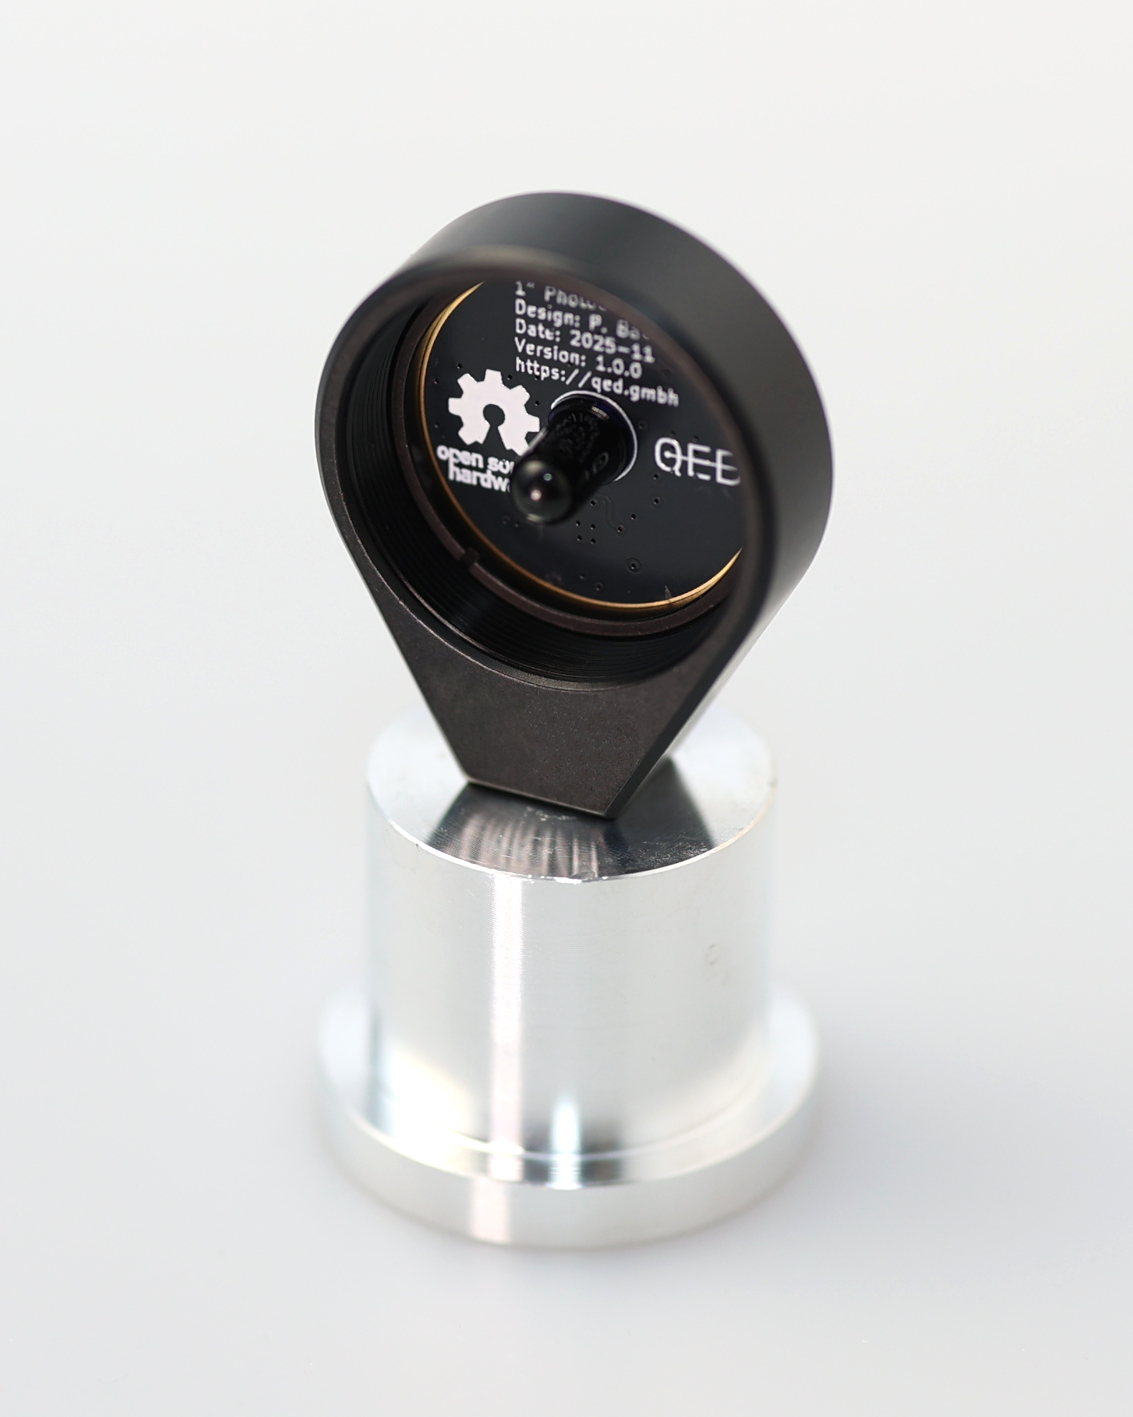
\includegraphics[width=6cm]{images/1inch-pd.jpg}
\end{figure}

Using a small footprint SMP connector the photodetecor can also be mounted in space constrained applications. The plug-and-play SMP connector ensures that the connector is always seated properly, eliminating noise caused by poor contacts.

% Switch to next column
\vfill\break

\tableofcontents

% For wide tables, a single column layout is better. It can be switched
% page-by-page.
\onecolumn

\section{Revision History}
\begin{table}[h]
    \centering
    \begin{tabularx}{\textwidth}{l| l | >{\raggedright\arraybackslash}X}
        \thickhline
        Version& Date& Comment\\
        \hline
        0.1.0 &2026-05-22 &Initial release. Compatible with hardware revision 1.0.0.\\
        \hline
        0.1.1 &2026-05-22 &Fixed QR-Code URL.\\
        \hline
        \versionNumber &2026-05-26 &Updated datasheet style to KOMA fixing page numbering.\\
        \thickhline
    \end{tabularx}
\end{table}

The latest release of this document can be found at \url{\repoUrl} or use the QR-code below.

\begin{center}
    \qrcode[nolinks]{\repoUrl}
\end{center}
\end{document}
